\documentclass{beamer}

\usepackage[utf8]{inputenc}
\usetheme{Madrid}


%%% macro %%%

\usepackage{amsfonts,amssymb}
\usepackage{graphicx}
\usepackage{epic}
\usepackage{biblatex}
\usepackage{soul}
\bibliography{ref.bib}

%%%%%%%%%%%%%%%%%%%%%%%%%%%%%%%%%%%%%%%%%%%%%%%%%%%%%%%%%%%%%%%%%%%%%%%%%%%%%%%
% Definitions

\newcommand{\<}{\langle}
\renewcommand{\>}{\rangle}

\newcommand{\be}{\begin{equation}}
\newcommand{\ee}{\end{equation}}
\newcommand{\bea}{\begin{eqnarray}}
\newcommand{\eea}{\end{eqnarray}}

\newcommand{\cond}[1]{\left\{\begin{array}{l@{~~~}l}#1\end{array}\right.}
\newcommand{\qph}[1]{quant-ph/#1}

\newcommand{\BPP}{{\mathrm{BPP}}}
\newcommand{\BQP}{{\mathrm{BQP}}}
\newcommand{\ent}{{\textsc{entrance}}}
\newcommand{\exit}{{\textsc{exit}}}
\renewcommand{\root}{{\textsc{root}}}

\renewcommand{\d}{{\mathrm{d}}}
\newcommand{\sech}{\mathop{\mathrm{sech}}\nolimits}
\newcommand{\Ai}{\mathop{\mathrm{Ai}}\nolimits}
\newcommand{\poly}{\mathop{\mathrm{poly}}\nolimits}
\newcommand{\col}{\mathop{\mathrm{col}}\nolimits}

\newcommand\symProb{\mathop{\mathrm{Pr}}\displaylimits}
\newcommand\symExpec{\mathop{\mathrm{E}}\displaylimits}
\def\prob#1#2{\symProb_{#1}\left[ #2 \right]}
\def\expec#1#2{\symExpec_{#1}\left[ #2 \right]}


%%%%%%%%%%%%%%%%%%%%%%%%%%%%%%%%%%%%%%%%%%%%%%%%%%%%%%%%%%%%%%%%%%%%%%%%%%%%%%%

%%% Info %%%

\title{Exponential algorithmic speedup by quantum walk}
\author{Yan-Tong Lin}
\institute{National Chiao Tung University}
\date{QIQC 2020fall, 2020/12/22}

\begin{document}

\AtBeginSection[]
{
  \begin{frame}
    \frametitle{}
    \setcounter{tocdepth}{3}
    \tableofcontents[currentsection, hideothersubsections]
  \end{frame}
}

\frame{\titlepage}

%%% Outline %%%

\begin{frame}
\frametitle{Outline}
\setcounter{tocdepth}{1}
\tableofcontents
\end{frame}

%%%%%%%%%%%%%%%%%%%%%%%%%%%%%%%%%%%%%%%%%%%%%%%%%%%%%%%%%%%%%

\section{Introduction} \label{sec:intro}

\begin{frame}{Previous Work}
    \begin{itemize}
        \item Quantum analogues to random walks were proposed 
        \item Separation was not "algorithmic"
    \end{itemize}
    \begin{figure}
        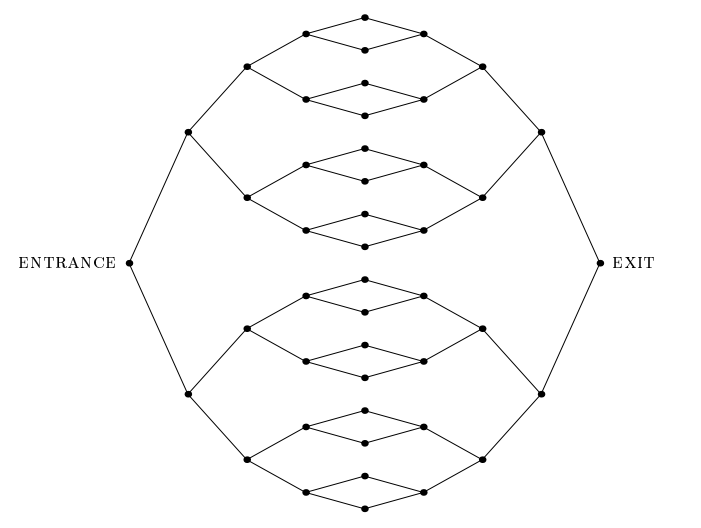
\includegraphics[width=0.6\textwidth]{basicgraph4.png}
        \caption{The graph $G_4$.}
        \label{fig:graph}
    \end{figure}
\end{frame}

\begin{frame}{This Paper}
Provide a graph where the separation is "algorithmic".
    \begin{figure}
        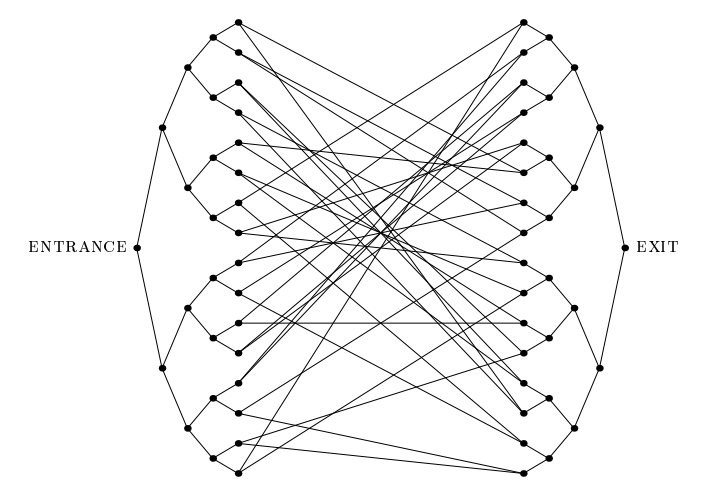
\includegraphics[width=0.7\textwidth]{graph4.png}
        \caption{A typical graph $G^{\prime}_4$.}
        \label{fig:graphprime}
    \end{figure}
\end{frame}

%%%%%%%%%%%%%%%%%%%%%%%%%%%%%%%%%%%%%%%%%%%%%%%%%%%%%%%%%%%%%

\section{The problem}\label{sec:problem}

\begin{frame}{The problem}
    \begin{block}{}
        \begin{itemize}
            \item Input: an oracle for the graph and the name of the $\ent$
            \item Output: find the name of the $\exit$
        \end{itemize}
    \end{block}
    
    \begin{exampleblock}{}
        \begin{itemize}
            \item number of vertex is $N$ and $n=O(\log(n))$
            \item names are $2n$-bit string
        \end{itemize}
    \end{exampleblock}
    
\end{frame}




%%%%%%%%%%%%%%%%%%%%%%%%%%%%%%%%%%%%%%%%%%%%%%%%%%%%%%%%%%%%%

\section{Quantum algorithm}\label{sec:algorithm}

\subsection{Quantum walk}\label{subsec:qwalk}

\begin{frame}{Classical Random Walk}
\begin{block}{Markov process}
    \be
      K_{aa'} = \cond{ 
          \gamma       & a \ne a', \ aa' \in G \\
          0            & a \ne a', \ aa' \notin G \\
          -d(a) \gamma & a=a' \,.}
    \ee
    \be
      {\d p_a(t) \over \d t} = \sum_{a'} K_{aa'} \, p_{a'}(t)
    \,.
    \label{eq:diffeq}
    \ee
here $\gamma$ is the probability to go to an adjacent vertex in a unit time.
\end{block}
\end{frame}

%%%

\begin{frame}{Quantum Analogue}

\begin{block}{the Schr\"odinger equation}
\be
  i {{\mathrm d} \over {\mathrm d}t} \<a|\psi(t)\> = \sum_{a'} \<a|H|a'\> \<a'|\psi(t)\>
\ee
\end{block}

\begin{block}{}
\begin{itemize}
    \item In \cite{FG98}, $\langle a | H | a^{\prime} \rangle = K_{aa^{\prime}}$
    \item In this paper, \be
  \<a|H|a'\> = \cond{ \gamma & a \ne a', \ aa' \in G \\
                      0      & \textrm{otherwise.} }
\label{eq:graphham}
\ee
\end{itemize}
\end{block}

\begin{alertblock}{}
For norm preserving, a Hamiltonian with Hermiticity is required.
\end{alertblock}

\begin{exampleblock}{Goal}
simulate the unitary evolution $e^{-i H t}$ with $H$ given by (\ref{eq:graphham})
\end{exampleblock}

\end{frame}

%%%

\note[itemize]{
\item Now consider quantum evolution in an N-dimensional Hilbert space spanned by states |1i, |2i,… , |Ni corresponding to the vertices of G. If the Hamiltonian is H, then the dynamics of the system are determined by the Schr¨odinger equation
}

\subsection{Implementing the quantum walk}\label{subsec:implement}

%%%

\begin{frame}{Implementing the quantum walk - the Oracle }

\begin{alertblock}{}
To make the oracle, an additional structure is required \newline 
a consistent $k$-edge coloring, here $k=\poly(\log N)$.
\end{alertblock}

\begin{definition}
An edge coloring is consistent if no vertex is incident with two edges of the same color.
\end{definition}

\begin{block}{Remark}
We will show that the oracle can provide a consistent coloring for the graph that cannot be used by any classical algorithm to help solve the problem, since a classical algorithm could make up the coloring as it goes. 
\end{block}

\end{frame}
%%%

\begin{frame}{Implementing the quantum walk - the Oracle (Cont.) }

\begin{block}{}
Given a consistent coloring, the graph is presented with the oracle $U$
\be
  U |a,b,c\> = |a,b \oplus v_c(a),c\>
\label{eq:graphoracle}
\ee
\begin{itemize}
    \item $a, b$ are $2n$-bit strings
    \item $c$ is a color
    \item $v_c(a) = a'$, $a'=11\ldots1$ if vertex $a$ doesn't exist or there is no incident edge of color $c$
    \item Note that  $v_c(v_c(a))=a$ for $v_c(a) \ne 11\ldots1$
    
\end{itemize}
\end{block}

\end{frame}

%%%

\begin{frame}{Implementing the quantum walk - the Oracle (Cont.) }
Since no query with a superposition of colors will be used and we want to track whether there is an $11\ldots1$ case, we construct oracle $V_c$ for each color $c$ with $U$.
\begin{block}{the final oracle}
\be
  V_c|a,b,r\> = |a,b \oplus v_c(a),r \oplus f_c(a)\>
\,,
\label{eq:simpleoracle}
\ee
where
\be
  f_c(a) = \cond{
      0 & v_c(a) \ne 11\ldots1 \\
      1 & v_c(a) = 11\ldots1 }
\ee
\end{block}
We will use $V_c$s to simulate the quantum evolution with Hamiltonian $H$
\be
  H |a, 0, 0\> = \sum_{c:\, v_c(a) \in G} |v_c(a),0,0\>
\,.
\label{eq:ham}
\ee

%%%

\end{frame}

\note[itemize]{
\item Nielson and Chuang p.204 
}

%%%

\begin{frame}{Useful standard tools for simulating Hamiltonians}
    
\begin{block}{Useful standard tools for simulating Hamiltonians}

\begin{enumerate}
    \item {\em Local terms.}
    \item {\em Linear combination.}
    \item {\em Unitary conjugation.} 
    \item {\em Tensor product.}  
\end{enumerate}    

\end{block}
    
\end{frame}

%%%

\begin{frame}{Simulating $H$}

\begin{block}{Hermitian operator $T$ }
\bea
  T |a, b, 0\> &=& |b, a, 0\> \\
  T |a, b, 1\> &=& 0
\,.
\eea
\end{block}
It is obvious that $V_c^\dag = V_c$ and
\be
  H = \sum_c V_c^\dag T V_c
\label{eq:simham}
\ee
So it remains to simulate $T$ efficiently.

\end{frame}

\begin{frame}{Simulating T}

The operator $T$ may be written as
\be
  T = \left( \bigotimes_{l=1}^{2n} S^{(l,2n+l)} \right) \otimes |0\>\<0|
\label{eq:swap}
\ee
$S |z_1 z_2\> = |z_2 z_1\>$, the superscript indicates which two qubits $S$ acts on.
\newline \newline
Observe that the eigenvalues of $S$ are $\pm1$, so the eigenvalues of $T$ are $0, \pm1$.
And an operator can be uniquely determined by its behavior on its eigenbasis. So $T$ is implemented with the circuit in Fig.\ref{fig:simT}.

\end{frame}

\begin{frame}{Simulating T II}

\begin{figure}
\setlength{\unitlength}{1.8pt}
\begin{picture}(180,105)
\put(10,5){\line(1,0){78}}
\put(102,5){\line(1,0){78}}
\put(10,15){\line(1,0){84}}
\put(96,15){\line(1,0){84}}
\put(10,25){\line(1,0){10}}
\put(40,25){\line(1,0){39}}
\put(81,25){\line(1,0){28}}
\put(111,25){\line(1,0){39}}
\put(170,25){\line(1,0){10}}
\put(10,35){\line(1,0){10}}
\put(40,35){\line(1,0){110}}
\put(170,35){\line(1,0){10}}
\put(10,65){\line(1,0){10}}
\put(40,65){\line(1,0){19}}
\put(61,65){\line(1,0){68}}
\put(131,65){\line(1,0){19}}
\put(170,65){\line(1,0){10}}
\put(10,75){\line(1,0){10}}
\put(40,75){\line(1,0){110}}
\put(170,75){\line(1,0){10}}
\put(10,90){\line(1,0){10}}
\put(40,90){\line(1,0){9}}
\put(51,90){\line(1,0){88}}
\put(141,90){\line(1,0){9}}
\put(170,90){\line(1,0){10}}
\put(10,100){\line(1,0){10}}
\put(40,100){\line(1,0){110}}
\put(170,100){\line(1,0){10}}
\put(20,85){\framebox(20,20){$W$}}
\put(20,60){\framebox(20,20){$W$}}
\put(20,20){\framebox(20,20){$W$}}
\put(150,85){\framebox(20,20){$W^\dag$}}
\put(150,60){\framebox(20,20){$W^\dag$}}
\put(150,20){\framebox(20,20){$W^\dag$}}
\put(50,5){\circle{4}}
\put(50,90){\circle{2}}
\put(50,100){\circle*{2}}
\put(50,100){\line(0,-1){9}}
\put(50,89){\line(0,-1){86}}
\put(60,5){\circle{4}}
\put(60,65){\circle{2}}
\put(60,75){\circle*{2}}
\put(60,75){\line(0,-1){9}}
\put(60,64){\line(0,-1){61}}
\put(80,5){\circle{4}}
\put(80,25){\circle{2}}
\put(80,35){\circle*{2}}
\put(80,35){\line(0,-1){9}}
\put(80,24){\line(0,-1){21}}
\put(110,5){\circle{4}}
\put(110,25){\circle{2}}
\put(110,35){\circle*{2}}
\put(110,35){\line(0,-1){9}}
\put(110,24){\line(0,-1){21}}
\put(130,5){\circle{4}}
\put(130,65){\circle{2}}
\put(130,75){\circle*{2}}
\put(130,75){\line(0,-1){9}}
\put(130,64){\line(0,-1){61}}
\put(140,5){\circle{4}}
\put(140,90){\circle{2}}
\put(140,100){\circle*{2}}
\put(140,100){\line(0,-1){9}}
\put(140,89){\line(0,-1){86}}
\put(95,15){\circle{2}}
\put(95,14){\line(0,-1){4}}
\put(88,0){\framebox(14,10){$e^{-iZt}$}}
\put(30,45){\circle*{1}}
\put(30,50){\circle*{1}}
\put(30,55){\circle*{1}}
\put(68,55){\circle*{1}}
\put(70,50){\circle*{1}}
\put(72,45){\circle*{1}}
\put(160,45){\circle*{1}}
\put(160,50){\circle*{1}}
\put(160,55){\circle*{1}}
\put(122,55){\circle*{1}}
\put(120,50){\circle*{1}}
\put(118,45){\circle*{1}}
\put(0,0){\makebox(10,10){$|0\rangle$}}
\put(0,10){\makebox(10,10){$r$}}
\put(0,20){\makebox(10,10){$b_{2n}$}}
\put(0,30){\makebox(10,10){$a_{2n}$}}
\put(0,60){\makebox(10,10){$b_2$}}
\put(0,70){\makebox(10,10){$a_2$}}
\put(0,85){\makebox(10,10){$b_1$}}
\put(0,95){\makebox(10,10){$a_1$}}
\end{picture}
\caption{A circuit for simulating $e^{-iTt}$.}
\label{fig:simT}
\end{figure}

\end{frame}

\begin{frame}{Simulating T III}

let $W$ be the two-qubit unitary operator that diagonalizes $S$.
\bea
  W |00\> &=& |00\> \\
  W {\textstyle{1 \over \sqrt2}}(|01\> + |10\>) &=& |01\> \\
  W {\textstyle{1 \over \sqrt2}}(|01\> - |10\>) &=& |10\> \\
  W |11\> &=& |11\>
\,.
\eea
$W^{\otimes 2n}$ diagonalizes $T$, and the Toffoli gates compute
the argument of the eigenvalue in an ancilla register initially prepared
in the state $|0\>$, and then apply the appropriate phase shift.

\end{frame}


%%%%%%%%%%%%%%%%%%

\subsection{Propagation on a line}\label{subsec:line}

\begin{frame}{Propagation on a line - Physics Intuition}
In the section, we use physics techniques to provide intuition that the quantum walk propagates from the $\ent$ to the $\exit$ in linear time. 
\newline 
\newline 
By introducing the {\em column space}, we show the walk on $G_n'$ can be viewed as a walk on a finite line with a defect at the center.
\newline
\newline 
For this presentation, we will go through the simplest case with infinite spaces and no defect and explain briefly why the defect and the boundaries do not significantly affect the walk.

\end{frame}

\begin{frame}[allowframebreaks]{Propagation on a line - Column Space}

\begin{block}{Column Space}
the $(2n+2)$-dimensional subspace spanned by the states
\be
  |\col j\> = {1 \over \sqrt N_j} \sum_{a \in \mathrm{column~} j} |a\>
\,,
\ee
where
\be
  N_j = \cond{2^j        &   0 \le j \le n \\
              2^{2n+1-j} & n+1 \le j \le 2n+1 \,.}
\ee
\end{block}

The column subspace is  invariant under $H$ (every vertex in column j is connected to the same number of vertices in column j + 1 and vice versa).

\framebreak

\begin{block}{$H$ in column space}
\be
  \<\col j|H|\col(j+1)\> = \cond{
   \sqrt 2 \gamma & 0 \le j \le n-1 \,,~~ n+1 \le j \le 2n \\
   2 \gamma       & j=n}
\label{eq:lineham}
\ee
\end{block}
For simplicity, we set $\gamma=1/\sqrt2$. 

\framebreak

\begin{figure}
\setlength{\unitlength}{1.2pt}
\begin{tabular}{r@{\hspace{18pt}}c}
\raisebox{16pt}{(a)} &
\begin{picture}(220,20)
\put(10,10){\circle*{2}}
\put(30,10){\circle*{2}}
\put(50,10){\circle*{2}}
\put(60,10){\circle*{.5}}
\put(65,10){\circle*{.5}}
\put(70,10){\circle*{.5}}
\put(80,10){\circle*{2}}
\put(100,10){\circle*{2}}
\put(120,10){\circle*{2}}
\put(140,10){\circle*{2}}
\put(150,10){\circle*{.5}}
\put(155,10){\circle*{.5}}
\put(160,10){\circle*{.5}}
\put(170,10){\circle*{2}}
\put(190,10){\circle*{2}}
\put(210,10){\circle*{2}}
\put(10,10){\line(+1,0){45}}
\put(75,10){\line(+1,0){70}}
\put(165,10){\line(+1,0){45}}
\put(15,10){\makebox(10,10){$1$}}
\put(35,10){\makebox(10,10){$1$}}
\put(85,10){\makebox(10,10){$1$}}
\put(105,10){\makebox(10,10){$\sqrt 2$}}
\put(125,10){\makebox(10,10){$1$}}
\put(175,10){\makebox(10,10){$1$}}
\put(195,10){\makebox(10,10){$1$}}
\put(-13,5){\makebox(20,10){\scriptsize $\ent$}}
\put(212,5){\makebox(10,10){\scriptsize $\exit$}}
\put(5,0){\makebox(10,10){\scriptsize $\col 0$}}
\put(25,0){\makebox(10,10){\scriptsize $\col 1$}}
\put(45,0){\makebox(10,10){\scriptsize $\col 2$}}
\put(75,0){\makebox(10,10){\scriptsize $\col n\!-\!1$}}
\put(95,0){\makebox(10,10){\scriptsize $\col n$}}
\put(115,0){\makebox(10,10){\scriptsize $\col n\!+\!1$}}
\put(135,0){\makebox(10,10){\scriptsize $\col n\!+\!2$}}
\put(165,0){\makebox(10,10){\scriptsize $\col 2n\!-\!1$}}
\put(185,0){\makebox(10,10){\scriptsize $\col 2n$}}
\put(205,0){\makebox(10,10){\scriptsize $\col 2n\!+\!1$}}
\end{picture}
\vspace{10pt}
\\ \raisebox{16pt}{(b)} &
\begin{picture}(160,20)
\put(10,10){\circle*{2}}
\put(30,10){\circle*{2}}
\put(50,10){\circle*{2}}
\put(70,10){\circle*{2}}
\put(90,10){\circle*{2}}
\put(110,10){\circle*{2}}
\put(130,10){\circle*{2}}
\put(150,10){\circle*{2}}
\put(10,10){\vector(+1,0){150}}
\put(10,10){\vector(-1,0){10}}
\put(15,10){\makebox(10,10){$1$}}
\put(35,10){\makebox(10,10){$1$}}
\put(55,10){\makebox(10,10){$1$}}
\put(75,10){\makebox(10,10){$1$}}
\put(95,10){\makebox(10,10){$1$}}
\put(115,10){\makebox(10,10){$1$}}
\put(135,10){\makebox(10,10){$1$}}
\end{picture}
\vspace{10pt}
\\ \raisebox{16pt}{(c)} &
\begin{picture}(160,20)
\put(10,10){\circle*{2}}
\put(30,10){\circle*{2}}
\put(50,10){\circle*{2}}
\put(70,10){\circle*{2}}
\put(90,10){\circle*{2}}
\put(110,10){\circle*{2}}
\put(130,10){\circle*{2}}
\put(150,10){\circle*{2}}
\put(10,10){\vector(+1,0){150}}
\put(10,10){\vector(-1,0){10}}
\put(65,0){\makebox(10,10){\scriptsize $j=d$}}
\put(85,0){\makebox(10,10){\scriptsize $j=d\!+\!1$}}
\put(15,10){\makebox(10,10){$1$}}
\put(35,10){\makebox(10,10){$1$}}
\put(55,10){\makebox(10,10){$1$}}
\put(75,10){\makebox(10,10){$\alpha$}}
\put(95,10){\makebox(10,10){$1$}}
\put(115,10){\makebox(10,10){$1$}}
\put(135,10){\makebox(10,10){$1$}}
\end{picture}
\vspace{10pt}
\\ \raisebox{16pt}{(d)} &
\begin{picture}(170,20)
\put(10,10){\circle*{2}}
\put(30,10){\circle*{2}}
\put(50,10){\circle*{2}}
\put(70,10){\circle*{2}}
\put(80,10){\circle*{.5}}
\put(85,10){\circle*{.5}}
\put(90,10){\circle*{.5}}
\put(100,10){\circle*{2}}
\put(120,10){\circle*{2}}
\put(140,10){\circle*{2}}
\put(160,10){\circle*{2}}
\put(10,10){\line(+1,0){65}}
\put(95,10){\line(+1,0){65}}
\put(5,0){\makebox(10,10){\scriptsize $j=1$}}
\put(155,0){\makebox(10,10){\scriptsize $j=L$}}
\put(15,10){\makebox(10,10){$1$}}
\put(35,10){\makebox(10,10){$1$}}
\put(55,10){\makebox(10,10){$1$}}
\put(105,10){\makebox(10,10){$1$}}
\put(125,10){\makebox(10,10){$1$}}
\put(145,10){\makebox(10,10){$1$}}
\end{picture}
\end{tabular}
\caption{Quantum walks on lines.
  (a) Reduction of the quantum walk on $G_n'$ to a quantum walk on a line.
  (b) Quantum walk on an infinite, translationally invariant line.
  (c) Quantum walk on an infinite line with a defect.
  (d) Quantum walk on a finite line without a defect.}
\label{fig:line}
\end{figure}

\end{frame}

%%%

\begin{frame}[allowframebreaks]{Propagation on a line - Infinite Line w/o Defects}

\begin{block}{Hamiltonian $H$ for an infinite line w/o defect}
\be
  \<j|H|j\pm 1\> = 1 \,,\quad -\infty < j < \infty
\,.
\ee
\end{block}
The eigenstates of this Hamiltonian are the momentum eigenstates $|p\>$ with components
\be
  \<j|p\> = {1 \over \sqrt{2\pi}} e^{i p j}
  \,, \quad -\pi \le p \le \pi
\ee
having energies
\be
  E_p = 2 \cos p 
\,.
\ee

\framebreak

\begin{block}{Propagator $G(j, k, t)$ from $j$ to $k$ in time $t$}
\bea
\label{eq:green}
  G(j,k,t) &=& \<k|e^{-i H t}|j\> \\
           &=& {1 \over 2 \pi} \int_{-\pi}^\pi \! \d p \, 
	       e^{i p (k-j) - 2 i t \cos p} \\
	   &=& (-i)^{k-j} J_{k-j}(2t) \,,\quad -\infty < j,k < \infty
\eea
where $J_\nu(\cdot)$ is a Bessel function of order $\nu$.
\newline
\end{block}
Note: here use $|j\> = \int_p |p\>\<p|j\>$

\framebreak

the Bessel function has the following asymptotic expansions for
$\nu \gg 1$:
\footnotesize
\bea
  J_\nu(\nu \sech \xi) 
    &\sim& {e^{-\nu(\xi-\tanh \xi)} \over \sqrt{2 \pi \nu \tanh \xi}} 
    \label{eq:besselahead} \\
  J_\nu(\nu+\xi\nu^{1/3}) 
    &=& (2/\nu)^{1/3} \Ai(-2^{1/3}\xi) + O(\nu^{-1})
    \label{eq:besseledge} \\
  J_\nu(\nu \sec \xi)
       &=& \sqrt{2 \over \pi \nu \tan\xi} \left\{
           \cos[\textstyle{\pi \over 4}-\nu(\xi-\tan \xi)] + O(\nu^{-1})
	   \right\}
           \,, \quad 0 < \xi < {\pi \over 2} \label{eq:besselbehind}
\eea
\normalsize

which means for $|k-j| \gg 1$
\[
 G(j, k, t) \text{ is } 
  \begin{cases} 
   \text{exponentially small in } |k-j| & \text{for } t <0.99\cdot |k-j|/2 \\
   \text{of order }|k-j|^{-1/3} & \text{ for }t\text{ near }|k-j|/2 \\
   \text{of order }|k-j|^{-1/2} & \text{ for }t >1.01\cdot |k-j|/2 \\
  \end{cases}
\]

\end{frame}

\subsection{Upper bound on the hitting time}\label{subsec:hitting}

\begin{frame}[allowframebreaks]{Upper bound on the hitting time --- Reflector and Commutablility}
\begin{block}{Recap --- the Hamiltonian for $G_{n-1}'$}
\be
  \<\col j|H|\col(j+1)\> = \cond{
   1      & 1 \le j \le n-1 \,,~~ n+1 \le j \le 2n-1 \\
   \sqrt2 & j=n \,,}
\ee
\end{block}

\begin{block}{Definition --- the Reflection Operator}
\be
  R|\col j\> = |\col(2n+1-j)\>
\,.
\ee
\end{block}
Note that $R^2=1$, so $R$ has eigenvalues $\pm 1$.  $R$ commutes with $H$
on the column subspace, so we can find simultaneous eigenstates of $R$ and
$H$. 

\framebreak

\begin{block}{simultaneous eigenstates of $R$ and
$H$. }

\be
  \<\col j|E\> = \cond{
    \sin p j          & 1 \le j \le n \\
    \pm\sin(p(2n+1-j)) & n+1 \le j \le 2n \,, }
\label{eq:eigenstates}
\ee

\end{block}
The eigenvalue corresponding to the eigenstate $|E\>$ is $E=2 \cos p$, and the
quantization condition (to be discussed later) comes from matching at
vertices $n$ and $n+1$.  The $\ent$ vertex corresponds to $|\col 1\>$ and
the $\exit$ vertex to $|\col 2n\>$.

\begin{alertblock}{Remark}
The proof of the lemma make use of the fact that $\<E|\col 1\>=\pm\<E|\col
2n\>$ so that one can bound the probability term easily. 
\end{alertblock}

\end{frame}

\begin{frame}[allowframebreaks]{Upper bound on the hitting time --- Linking Success Probability to Spectral Gap}

\begin{lemma}\label{lemma:hitting}
Consider the quantum walk in $G_{n-1}'$ starting at the $\ent$.  Let the
walk run for a time $t$ chosen uniformly in $[0,\tau]$ and then measure in
the computational basis.  If $\tau \ge {4n \over \epsilon \, \Delta E}$
for any constant $\epsilon>0$, where $\Delta E$ is the magnitude of the
smallest gap between any pair of eigenvalues of the Hamiltonian, then the
probability of finding the $\exit$ is greater than ${1 \over
2n}(1-\epsilon)$.
\end{lemma}

\end{frame}

\begin{frame}[allowframebreaks]{Upper bound on the hitting time --- Proof for Lemma 1}

\small

The probability of finding the $\exit$ after the randomly chosen time $t
\in [0,\tau]$ is
\bea
  && {1 \over \tau} \int_0^\tau \! \d t \,
     |\<\col 2n|e^{-i H t}|\col 1\>|^2 \nonumber\\
  &&\qquad = \, {1 \over \tau} \sum_{E,E'} \int_0^\tau \! \d t \, 
                e^{-i(E-E')t} \<\col 2n|E\>\<E|\col 1\> 
                              \<\col 1|E'\>\<E'|\col 2n\> \\
  &&\qquad = \, \sum_E |\<E|\col 1\>|^2 |\<E|\col 2n\>|^2 \nonumber\\
  &&\qquad ~ \,\, + \sum_{E \ne E'} {1 - e^{-i(E-E')\tau} \over i(E-E')\tau}
	      \<\col 2n|E\>\<E|\col 1\> \<\col 1|E'\>\<E'|\col 2n\>
\,.
\eea
Because of (\ref{eq:eigenstates}), we have $\<E|\col 1\>=\pm\<E|\col
2n\>$.  Thus the first term is
\be
  \sum_E |\<E|\col 1\>|^4 \ge {1 \over 2n}
\ee
as is easily established using the Cauchy-Schwartz inequality.  The second
term can be bounded as follows:
\bea
  && \left |\sum_{E \ne E'} {1 - e^{-i(E-E')\tau} \over i(E-E')\tau}
           \<\col 2n|E\>\<E|\col 1\> 
           \<\col 1|E'\>\<E'|\col 2n\> \right| \nonumber\\
  && \qquad \le {2 \over \tau \Delta E} 
     \sum_{E,E'} |\<E|\col 1\>|^2 |\<E'|\col 2n\>|^2
    ={2 \over \tau \Delta E}
\,.
\eea
Thus we have
\be
  {1 \over \tau} \int_0^\tau \! \d t \, |\<\col 2n|e^{-i H t}|\col 1\>|^2
  \ge {1 \over 2n} - {2 \over \tau \Delta E}
  \ge {1 \over 2n} (1-\epsilon)
\ee
where the last inequality follows since $\tau \ge {4 n \over \epsilon \,
\Delta E}$ by assumption.

\normalsize

\end{frame}

%%%%%%%%%%%%Bounding the spectral gaps%%%%%%%%%%%%%

\begin{frame}[allowframebreaks]{Upper bound on the hitting time --- Bounding the spectral gaps}

\begin{lemma}\label{lemma:gap}
The smallest gap between any pair of eigenvalues of the Hamiltonian
satisfies
\be
  \Delta E > {2 \pi^2 \over (1+\sqrt2)n^3} + O(1/n^4)
\,.
\ee
\end{lemma}

\end{frame}

\begin{frame}[allowframebreaks]{Upper bound on the hitting time --- Proof of Lemma 2}
To evaluate the spacings between eigenvalues, we need to use the
quantization condition.  We have
\be
  \<\col n|H|E\> = 2 \cos p \, \<\col n|E\>
\ee
so that
\be
  \sqrt2 \<\col(n+1)|E\> + \<\col(n-1)|E\> = 2 \cos p \, \<\col n|E\>
\ee
and using (\ref{eq:eigenstates}), we have
\be
  \pm \sqrt2 \sin np + \sin((n-1)p) = 2 \cos p \, \sin np
\ee
which simplifies to
\be
  {\sin((n+1)p) \over \sin np} = \pm \sqrt 2
\,.
\label{eq:constraint}
\ee
In Figure \ref{fig:constraint} we plot the left hand side of
(\ref{eq:constraint}) for $n=5$.  The intersections with $-\sqrt2$ occur
to the left of the zeros of $\sin np$, which occur at $\pi l/n$ for
$l=1,2,\ldots,n-1$.  For the values of $p$ that intersect $-\sqrt 2$, we
can write $p=(\pi l/n)-\delta$.  Equation (\ref{eq:constraint}) with
$-\sqrt2$ on the right hand side is now
\be
  -\sqrt2 \sin n\delta = \sin\left(n\delta - {l\pi \over n} + \delta\right)
\,.
\label{eq:minus}
\ee
Write $\delta = (c/n) + (d/n^2) + O(1/n^3)$.  Taking $n\to\infty$ in
(\ref{eq:minus}) gives $-\sqrt2 \sin c = \sin c$, which implies that
$c=0$.  We then get
\be
  -\sqrt2 \sin\left({d \over n}+O(1/n^2)\right) 
        = \sin\left({d \over n}-{l \pi \over n}+O(1/n^2)\right)
\ee
which gives, as $n\to\infty$,
\be
  d = {l \pi \over 1+\sqrt 2}
\,.
\ee
Thus we have that the roots of (\ref{eq:constraint}) with $-\sqrt2$ on the
right hand side are of the form
\be
  p = {l \pi \over n} - {l \pi \over (1+\sqrt 2)n^2} + O(1/n^3)
\,.
\ee

\framebreak

\begin{figure}
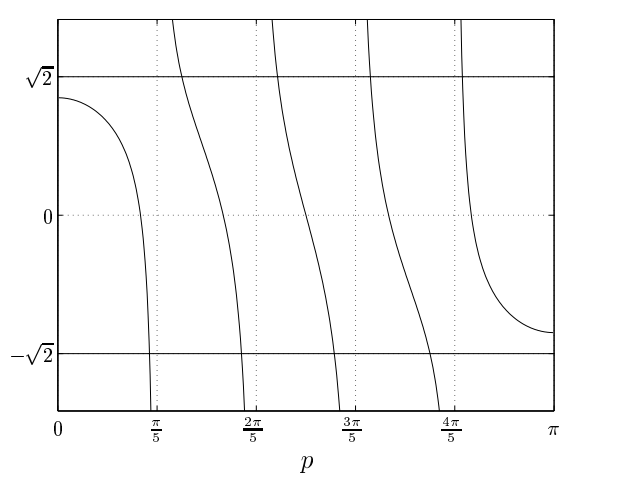
\includegraphics[width=0.7\textwidth]{cons.png}
\caption{Left hand side of (\ref{eq:constraint}) for $n=5$.}
\label{fig:constraint}
\end{figure}

\framebreak

Let $p'$ and $p''$ be the two roots of (\ref{eq:constraint}) closest to
the root $p$ just found, with $p' < p < p''$.  From the figure we see that
$p'$ and $p''$ both are roots of (\ref{eq:constraint}) with $+\sqrt2$.
(Note that the smallest $p$, corresponding to $l=1$, does not have a
$p'$.)   We see that $p''$ lies to the right of the zero of $\sin np$ at
$p=l\pi/n$.  We also see that $p'$ lies to the left of the zero of
$\sin((n+1)p)$ at $l \pi/(n+1)$.  Therefore we have
\bea
  p'  &<& {l \pi \over n} - {l \pi \over n^2} + O(1/n^3) \\
  p'' &>& {l \pi \over n}
\,,
\eea
from which we conclude that
\bea
  p-p'  &>& {l \pi \sqrt 2 \over (1+\sqrt2)n^2} + O(1/n^3) 
            \,, \quad l=2,3,\ldots,n-1 \\
  p''-p &>& {l \pi \over (1+\sqrt2)n^2} + O(1/n^3)
            \,, \quad l=1,2,\ldots,n-1
\,.
\eea
Thus the smallest spacing is at least $\pi/[(1+\sqrt2)n^2] + O(1/n^3)$.

Now for a given $p$, the corresponding eigenvalue is $2\cos p$.  For small
$\Delta p$, the spacing $\Delta E$ is related to the spacing $\Delta p$ by
\be
  \Delta E = 2 |\Delta p \, \sin p| + O\left((\Delta p)^2\right)
\,.
\ee
The factor $\sin p = \sin(l\pi/n + O (1/n^2))$ is smallest when $l=1$, so
we have
\be
  \Delta E > {2 \pi^2 \over (1+\sqrt 2) n^3} + O(1/n^4) > {8 \over n^3}
  \textrm{~ for $n$ sufficiently large.}
\ee

\framebreak


Notice that there are actually $10$ eigenvalues.
we can find two other eigenvalues at $\pm(\sqrt 2+{1 \over \sqrt 2})$ with
corrections that vanish exponentially as $n\to\infty$.  Since the other
$n-2$ eigenvalues are all in the range $[-2,2]$, our conclusion about the
minimum spacing is unchanged.

\begin{alertblock}{Remark}
The proof is sketched as follow. First, find the plotting to gain intuition of the solutions. Then, use distance to $\frac{l\pi}{n}$ to bound $\Delta p$. Finally, use $\Delta p$ to bind $\Delta E$
\end{alertblock}

\end{frame}

%%%

\begin{frame}{Upper bound on the hitting time --- Conclusion}

Using Lemma \ref{lemma:hitting} and Lemma \ref{lemma:gap}, we find
%
\begin{theorem}
For $n$ sufficiently large, running the quantum walk for a time chosen
uniformly in $[0,{n^4 \over 2\epsilon}]$ and then measuring in the
computational basis yields a probability of finding the $\exit$ that is
greater than ${1 \over 2n} (1-\epsilon)$.
\label{thm:hitting}
\end{theorem}

\begin{block}{An Efficient Quantum Algorithm for Traversing $G_n'$s}
The computer is prepared in the state corresponding to the $\ent$, and the quantum walk is simulated using the construction described in Section \ref{subsec:implement}.  After
running the walk for an appropriate $t=\poly(n)$, the state of the computer is
measured. The probability of finding the name of the $\exit$ can be $O(1/n)$.  By
repeating this process $\poly(n)$ times, the success probability can be
made arbitrarily close to 1. 
\end{block}

\end{frame}


%%%%%%%%%%%%%%%%%%%%%%%%%%%%%%%%%%%%%%%%%%%%%%%%%%%%%%%%%%%%%

\section{Classical lower bound}\label{sec:lowerbound}

\subsection{Overview}\label{classical:overview}

\begin{frame}{Classical lower bound --- Overview}

\begin{block}{{Claim}}
No classical algorithm can find the $\exit$ with high
probability in subexponential time.
\end{block}
We proof this by considering a series of games and proving relations between them. The first game is equivalent to our problem, and each new game will be as easy to win.
Finally, we will show that the easiest game cannot be won in subexponential time.
\end{frame}

\subsection{Coloring}\label{classical:coloring}
\begin{frame}{Classical lower bound --- Coloring}
To prove the classical lower bound, we need to specify a coloring that does not supply information about the graph.
\begin{block}{Algorithm for a consistent coloring}
In an even numbered column, randomly color the incident edges $A,B,C$.
In an odd numbered column, randomly append the colors of the incident edges $1,2,3$.
\end{block}
It is obvious that any such coloring is consistent. 
And we will show it does not provide any useful information to a classical algorithm.
\end{frame}

\subsection{Reduction to a Simpler Game}\label{classical:reduction}

\begin{frame}{Classical lower bound --- Reduction}

\begin{block}{Restrict to Known Vertices}
Since we have $2$-n bit string name, which means the probability of guessing a unknown name yield a valid vertex name is exponentially small.
\end{block}

\begin{block}{Removal of Coloring}
The coloring of graph can be made by the classical algorithm itself. 
For by restricting the explored subgraph to be connected, we know the parity of the column a vertex is in.
So it does not gain additional information about the graph with the coloring.
\end{block}

\begin{block}{Adding Win Condition --- Finding a Cycle}
Note the only information we have is the parity of the column of vertices, extra information cannot be gained unless we find a cycle. Thus we define a easier to win game that the player $A$ wins if it finds the $\exit$ or \textcolor{red}{it finds a cycle}. 
\end{block}

\end{frame}

\subsection{Linking to a Tree Embedding Problem}\label{classical:tree embedding}

\begin{frame}[allowframebreaks]{Classical lower bound --- Linking to Random Tree Embedding}

We show the subgraph an algorithm sees must be a random embedding of a rooted binary tree.

\begin{block}{Tree Embedding into $G$}
 $\pi : T \to G$ such that $\pi(\root) = \ent$ and for all vertices $u$ and $v$ that are neighbors in $T$, $\pi(u)$ and $\pi(v)$ are neighbors in $G$.
We say that an embedding of $T$ is {\em proper} if $\pi(u) \not = \pi(v)$ for $u \ne v$.
\end{block}

\begin{block}{Random Embedding for a Tree into $G$}
A random embedding of a tree is obtained by setting $\pi(\root) = \ent$ and then mapping the rest of $T$ into $G$ at random. (with prob $\frac12$ take $(u,v)$ or $(v,u)$)
\end{block}
\framebreak

\begin{block}{Embedding Game}\label{game:randomembedding}
The algorithm outputs a rooted binary tree $T$ with $t$ vertices in
which each internal vertex has two children.  A random $\pi$ is chosen.
The algorithm wins if $\pi$ is an improper embedding of $T$ in $G_n'$ or
if $T$ exits $G_n'$ under $\pi$.
\end{block}

\framebreak

\begin{block}{$\frac n2$ subtrees}
Let $T$ be a tree with $t$ vertices, $t \le 2^{n/6}$, with image $\pi(T)$
in $G_n'$ under the random embedding $\pi$.  The vertices of columns $n+1, n+2,
\ldots n+{n \over 2}$ in $G_n'$ divide naturally into $2^{n/2}$ complete
binary subtrees of height $n/2$.
\end{block}

It is very unlikely that $\pi(T)$ contains the root of any of these subtrees.  Consider a path in $T$ from the root to a leaf.  The path has length at most $t$, and there are at most $t$ such paths.  To reach column $n+{n\over 2}$ from column $n+1$, $\pi$ must choose to move right ${n \over
2}-1$ times in a row, which has probability $2^{1-n/2}$. The probability is bounded by
$t^2 \cdot 2^{1-n/2}$.

\framebreak

\begin{columns}
    \begin{column}{0.48\textwidth}
        If $\pi(T)$ contains a cycle, $\exists a,b \in T \ni \pi(a)=\pi(b)$. Consider $c=\textrm{LCA}(a,b)$, $\pi(c\to a), \pi(c\to b)$ forms a cycle. The probability of $a,b$ exceed the two $\frac n2$ lines is low. For forming a cycle, $P$(path to $a,b$ ends in the same subtree) $\le \frac{2^{\frac n 2}}{2^n-t}$ (by the construction of $G$, it is equally possible to pass any of the vertices in the $n$th column). We have to consider $\binom{t}{2}$ $a, b$ pairs.
    \end{column}
    \begin{column}{0.48\textwidth}
%%%
\begin{figure}
\setlength{\unitlength}{0.7pt}
\begin{picture}(150,220)
\drawline(65,0)(65,40)
\drawline(35,20)(65,40)
\drawline(35,20)(65,0)
\drawline(65,50)(65,90)
\drawline(35,70)(65,90)
\drawline(35,70)(65,50)
\drawline(65,120)(65,160)
\drawline(35,140)(65,160)
\drawline(35,140)(65,120)
\drawline(65,170)(65,210)
\drawline(35,190)(65,210)
\drawline(35,190)(65,170)
\drawline(85,0)(85,40)
\drawline(115,20)(85,40)
\drawline(115,20)(85,0)
\drawline(85,50)(85,90)
\drawline(115,70)(85,90)
\drawline(115,70)(85,50)
\drawline(85,120)(85,160)
\drawline(115,140)(85,160)
\drawline(115,140)(85,120)
\drawline(85,170)(85,210)
\drawline(115,190)(85,210)
\drawline(115,190)(85,170)
\put(50,98){\circle*{.75}}
\put(50,105){\circle*{.75}}
\put(50,112){\circle*{.75}}
\put(100,98){\circle*{.75}}
\put(100,105){\circle*{.75}}
\put(100,112){\circle*{.75}}
\put(15,130){\circle*{2}}
\put(57,135){\circle*{2}}
\dashline{2}(15,130)(55,190)
\dashline{2}(55,190)(95,140)
\dashline{2}(95,140)(57,135)
\dottedline{1}(57,135)(95,65)
\dottedline{1}(95,65)(45,20)
\dottedline{1}(45,20)(15,130)
\put(3,125){\makebox(10,10){\tiny $\pi(c)$}}
\put(35,115){\makebox(10,10){\tiny $\pi(a)=\pi(b)$}}
\put(47,125){\vector(1,1){7}}
\put(21,155){\makebox(10,10){\tiny $\pi(P_1)$}}
\put(14,80){\makebox(10,10){\tiny $\pi(P_2)$}}
\put(0,210){\makebox(10,10){\tiny$0$}}
\put(30,210){\makebox(10,10){\tiny$n \over 2$}}
\put(60,210){\makebox(10,10){\tiny$n$}}
\put(80,210){\makebox(10,10){\tiny$n+1$}}
\put(110,210){\makebox(10,10){\tiny$n+{n \over 2}$}}
\put(140,210){\makebox(10,10){\tiny$2n+1$}}
\end{picture}
\label{fig:subtrees}
\end{figure}
%%%
    \end{column}
\end{columns}

\normalsize

\framebreak

Overall we have shown that
\bea
  \expec{G}{\mathbb{P}^G(T)} 
    &\le& t^2 \cdot 2^{-n/2} + t^2 \cdot 2^{1-n/2} \\
    &\le& 3 \cdot 2^{-n/6}
\eea
if $t \le 2^{n/6}$.

\end{frame}

%%%%%%%%%%%%%%%%%%%%%%%%%%%%%%%%%%%%%%%%%%%%%%%%%%%%%%%%%%%%%

\section{Discussion}\label{sec:discussion}


\begin{frame}{Discussion}
    \begin{itemize}
        \item Exponential quantum-classical separation with quantum walks
        \item A new oracle relative to $\BQP \overset{?}= \BPP$
        \item The path is not found along with $\exit$ 
        \item Open Problems
            \begin{itemize}
                \item General graph oracles w/o coloring?
                \item Applications?
            \end{itemize}
    \end{itemize}
\end{frame}

%%%%%%%%%%%%%%%%%%%%%%%%%%%%%%%%%%%%%%%%%%%%%%%%%%%%%%%%%%%%%

\begin{frame}[allowframebreaks]
    \frametitle{References}
    \begin{thebibliography}{}
        \bibitem{Deu85}
          D. Deutsch, 
          {\em Quantum theory, the Church-Turing principle, and the universal
          quantum computer},
          Proc. Roy. Soc. London A {\bf 400}, 97 (1985).
        \bibitem{DJ92}
          D. Deutsch and R. Jozsa, 
          {\em Rapid solution of problems by quantum computation}, 
          Proc. Roy. Soc.  London A {\bf 439}, 553 (1992).
        \bibitem{BV93}
          E. Bernstein and U. Vazirani,
          {\em Quantum complexity theory}, 
          Proc. 25th ACM Symposium on the Theory of Computing, 11 (1993).
        \bibitem{Sim94}
          D. Simon,
          {\em On the power of quantum computation},
          Proc. 35th IEEE Symposium on the Foundations of Computer Science,
          116 (1994).
        \bibitem{Sho94}
          P. W. Shor,
          {\em Algorithms for quantum computation: discrete logarithms and
          factoring},
          Proc. 35th IEEE Symposium on Foundations of Computer Science, 124
          (1994).
        \bibitem{Kit95}
          A. Kitaev,
          {\em Quantum measurements and the abelian stabilizer problem},
          \qph{9511026}.
        \bibitem{ME99}
          M. Mosca and A. Ekert,
          {\em The hidden subgroup problem and eigenvalue estimation on a quantum
          computer},
          Proc. 1st NASA International Conference on Quantum Computing and Quantum
          Communication, Vol. 1509 of {\em Lecture Notes in Computer Science}
          (1999).
        \bibitem{BCW00}
          J. N. de Beaudrap, R. Cleve, and J. Watrous,
          {\em Sharp quantum vs. classical query complexity separations},
          \qph{0011065}.
        \bibitem{DH00}
          W. van Dam and S. Hallgren,
          {\em Efficient quantum algorithms for shifted quadratic character
          problems},
          \qph{0011067}.
        \bibitem{HRT00}
          S. Hallgren, A. Russell, and A. Ta-Shma,
          {\em Normal subgroup reconstruction and quantum computation using group
          representations},
          Proc. 32nd ACM Symposium on the Theory of Computing, 627 (2000).
        \bibitem{DHI01}
          W. van Dam, S. Hallgren, and L. Ip,
          {\em Quantum algorithms for hidden coset problems},
          unpublished.
        \bibitem{GSVV01}
          M. Grigni, L. Schulman, M. Vazirani, and U. Vazirani,
          {\em Quantum mechanical algorithms for the nonabelian hidden subgroup
          problem},
          Proc. 33rd ACM Symposium on the Theory of Computing,
          68 (2001).
        \bibitem{IMS01}
          G. Ivanos, F. Magniez, and M. Santha,
          {\em Efficient quantum algorithms for some instances of the non-abelian
          hidden subgroup problem},
          \qph{0102014}.
        \bibitem{Wat01}
          J. Watrous,
          {\em Quantum algorithms for solvable groups},
          Proc. 33rd ACM Symposium on the Theory of Computing, 60 (2001).
        \bibitem{Hal02}
          S. Hallgren,
          {\em Polynomial-time quantum algorithms for Pell's equation and the
          principal ideal problem},
          Proc. 34th ACM Symposium on the Theory of Computing, 653 (2002).
        \bibitem{FG98}
          E. Farhi and S. Gutmann,
          {\em Quantum computation and decision trees},
          Phys. Rev. A {\bf 58}, 915 (1998).
        \bibitem{CFG02}
          A. M. Childs, E. Farhi, and S. Gutmann,
          {\em An example of the difference between quantum and classical random
          walks},
          Quantum Information Processing {\bf 1}, 35 (2002).
        \bibitem{ADZ93}
          Y. Aharonov, L. Davidovich, and N. Zagury,
          {\em Quantum random walks},
          Phys. Rev. A {\bf 48}, 1687 (1993).
        \bibitem{Mey96}
          D. A. Meyer, 
          {\em From quantum cellular automata to quantum lattice gasses}, 
          J. Stat. Phys. {\bf 85}, 551 (1996).
        \bibitem{Wat01b}
          J. Watrous, 
          {\em Quantum simulations of classical random walks and undirected 
          graph connectivity},
          J. Computer and System Sciences {\bf 62}, 376 (2001).
        \bibitem{AAKV01}
          D. Aharonov, A. Ambainis, J. Kempe, and U. Vazirani, 
          {\em Quantum walks on graphs}, 
          in Proceedings of the 33rd ACM Symposium on the Theory of Computing, 50
          (ACM Press, New York, 2001).
        \bibitem{NV01}
          A. Ambainis, E. Bach, A. Nayak, A. Vishwanath, and J. Watrous, 
          {\em One-dimensional quantum walks}, 
          Proc. 33rd ACM Symposium on the Theory of Computing, 37 (ACM Press, New
          York, 2001).  
        \bibitem{MR01}
          C. Moore and A. Russell,
          {\em Quantum walks on the hypercube},
          \qph{0104137}.
        \bibitem{Kem02}
          J. Kempe,
          {\em Quantum random walks hit exponentially faster},
          \qph{0205083}.
        \bibitem{Viz64}
          V. G. Vizing,
          {\em On an estimate of the chromatic class of a $p$-graph}, Diskret.
          Analiz {\bf 3}, 23 (1964).
        \bibitem{Llo96}
          S. Lloyd,
          {\em Universal quantum simulators},
          Science {\bf 273}, 1073 (1996).
        \bibitem{NC00}
          M. A. Nielsen and I. L. Chuang,
          {\em Quantum Computation and Quantum Information}
          (Cambridge University Press, Cambridge, 2000).
        \bibitem{AS72}
          M. Abramowitz and I. A. Stegun, 
          {\em Handbook of Mathematical Functions}
          (Dover, New York, 1972).
        \bibitem{GoldComm}
          J. Goldstone, personal communication, September 2002.
    \end{thebibliography}
\end{frame}

\end{document}